%%%%%%%%%%%%%%%%%%%%%%%%%%%%%%%%%%%%%%%%%
% FRI Data Science_report LaTeX Template
% Version 1.0 (28/1/2020)
%
% Jure Demšar (jure.demsar@fri.uni-lj.si)
%
% Based on MicromouseSymp article template by:
% Mathias Legrand (legrand.mathias@gmail.com)
% With extensive modifications by:
% Antonio Valente (antonio.luis.valente@gmail.com)
%
% License:
% CC BY-NC-SA 3.0 (http://creativecommons.org/licenses/by-nc-sa/3.0/)
%
%%%%%%%%%%%%%%%%%%%%%%%%%%%%%%%%%%%%%%%%%


%----------------------------------------------------------------------------------------
%	PACKAGES AND OTHER DOCUMENT CONFIGURATIONS
%----------------------------------------------------------------------------------------
\documentclass[fleqn,moreauthors,10pt]{ds_report}
\usepackage[english]{babel}
\usepackage{multicol}
\usepackage{multirow}
\graphicspath{{fig/}}




%----------------------------------------------------------------------------------------
%	ARTICLE INFORMATION
%----------------------------------------------------------------------------------------

% Header
\JournalInfo{UL FRI Data Science - Natural Language Processing, 2022-2023}

% Interim or final report
%\Archive{Interim report}
\Archive{Project Report}

% Article title
\PaperTitle{Paraphrasing sentences in Slovene}

% Authors and their info
\Authors{Drejc Pesjak\textsuperscript{1}, Ilija Tavchioski\textsuperscript{2}, Klemen Vovk\textsuperscript{3}}
\affiliation{\textsuperscript{1}\textit{dp8949@student.uni-lj.si, 63180224} \textsuperscript{2}\textit{it8816@student.uni-lj.si, 63180383} \textsuperscript{3}\textit{kv4582@student.uni-lj.si, 63190317}}

% Multiple authors
%\Authors{John Doe\textsuperscript{1}, Jane Doe\textsuperscript{2}, and Mike Smith\textsuperscript{3}}
%\affiliation{\textsuperscript{1}\textit{john.doe@fri.uni-lj.si, 63181234}}
%\affiliation{\textsuperscript{1}\textit{jane.doe@fri.uni-lj.si, 63185678}}
%\affiliation{\textsuperscript{1}\textit{mike.smith@fri.uni-lj.si, 63171234}}

% Keywords
\Keywords{Natural Language Processing, Sentence paraphrasing, Transformers}
\newcommand{\keywordname}{Keywords}


%----------------------------------------------------------------------------------------
%	ABSTRACT
%----------------------------------------------------------------------------------------

\Abstract{
With the exponential growth of the natural language processing field using deep learning methods, especially transformers, we can see many \textit{state-of-the-art} models that have great performance on various tasks such as sentiment analysis, machine translation, text generation, sentence paraphrasing, and others. However, most of these methods are trained and used only on data written in English, our research goal is to develop a method for sentence paraphrasing in Slovenian language. We fine-tuned an already pre-trained GPT model (the Slovenian variant) on Slovenian data, and achieved promising performance on our test data, while also having a high average grade from human evaluators. Although the model performance is not yet production ready, it is a valid starting point to enrich the family of transformer-based models to other languages such as Slovenian.
}

%----------------------------------------------------------------------------------------

\begin{document}

% Makes all text pages the same height
\flushbottom

% Print the title and abstract box
\maketitle

% Removes page numbering from the first page
\thispagestyle{empty}

%----------------------------------------------------------------------------------------
%	ARTICLE CONTENTS
%----------------------------------------------------------------------------------------

\section*{Introduction}
The task of paraphrasing sentences is to change the original sentence while preserving the meaning it conveys. For example, \textit{Elephants consume small plants, bushes, fruit, and they can consume up to 170 kilograms of food per day.} can be paraphrased to \textit{An elephant can eat up to 170 kilograms of small plants, bushes and fruit per day.}. Paraphrasing can be used to aid machine translation, improve question answering \cite{paraphrasingtoimproveqa}, detect plagiarism and origin \cite{paraphrasestodetectorigin}, and evaluate machine-generated text (i.e. summaries) \cite{paraphrasestoevaluatetext}. This task has been greatly aided by the boom of deep learning (mainly transformers \cite{vaswani2017attention}). In this work, we tackle paraphrasing Slovene sentences by fine-tuning a large language model on a dataset of Slovene original and paraphrased sentences that have been obtained by translation from English, as there is vastly more (labeled) data available in English. 
%------------------------------------------------

\section*{Related work}
In related work, we can find several approaches to paraphrasing sentences in English and also in other languages as well. Mentioned are rule-based approaches \cite{mckeown-1979-paraphrasing} and translation-based approaches \cite{10.3115/1073012.1073020} which are the most common today, including paraphrasing with monolingual data, (two corpora: one is in English and of high quality, and the other is translated to Slovenian.). We leverage the English corpus to train the model to understand the relationship between paraphrases and then use the Slovenian corpus to teach the model to use the learned relationships to generate paraphrases in Slovenian.
\par
In addition, similar methods are developed using bilingual corpora \cite{mallinson-etal-2017-paraphrasing} where the paraphrase is determined by shared translation between the languages. On the other hand, with the rise of transformers \cite{vaswani2017attention} we can find several approaches using generative models such as GPT-2 \cite{DBLP:journals/corr/abs-1911-09661} where the model is fine-tuned on a predefined dataset with paraphrasing examples and performs with decent results. In addition, there are some approaches using other techniques such as deep reinforcement learning as well \cite{li-etal-2018-paraphrase}.


\section*{Methodology}

In this section, we describe the methodology we used for the task of paraphrasing Slovene sentences.

\subsection*{Dataset creation}

\subsubsection*{Sentence similarity in machine translation dataset}
We explored different methods to create a dataset suitable for fine-tuning a Language Model (LM). One of the approaches we considered was using a machine translation dataset. Specifically, we used the cjvt/rsdo4\_en\_sl dataset \cite{rsdo4_en_sl}, which consists of one million translated sentences from English to Slovene. Our goal was to find similar sentences in English and extrapolate their Slovene counterparts, thereby creating a parallel dataset for training our LM.

To achieve this, we used cosine distance on BERT embeddings \cite{reimers-2019-sentence-bert} to measure the similarity between sentences in English and Slovene. We found that despite using a state-of-the-art language model, the results were not satisfactory. Out of the first 10,000 sentences, only 200 pairs had a similarity score higher than 95\%. This was not sufficient for fine-tuning a LM, as we required a larger dataset to improve the performance of our model. Therefore, we concluded that using a machine translation dataset alone was not effective in creating a high-quality parallel corpus.

\subsubsection*{Slovene paraphrasing with GPT prompting}
Another approach we tried for creating a Slovene paraphrasing dataset was using GPT prompting. We used the cvjt/gpt-sl-base model \cite{huggingface_gptslbase} to generate paraphrases for the given input sentence. To do this, we prompted the GPT model to complete the original sentence with a paraphrased version. For instance, given the input sentence "Today is a beautiful day," we prompted the model with the phrase "\{input\_sentence\}, oziroma drugače," which translates to "\{input\_sentence\}, or in other words."

We found that this approach produced some promising results, with the GPT model generating a range of plausible paraphrased sentences for a given input. However, this approach suffered from the slow speed of generation. The cvjt/gpt-sl-base model \cite{huggingface_gptslbase} is a large language model with more than 125 million parameters, and generating paraphrases for a single sentence could take up to several minutes. Additionally, it was sometimes challenging to determine where the GPT model ended the paraphrased sentence. This made it challenging to identify the start and end points of the generated paraphrase, making it challenging to create a high-quality dataset. In the end, not enough data could be generated so we abandoned this method and considered premade datasets.

\subsubsection*{Machine translation of a paraphrase dataset}
The ParaBank2 dataset \cite{hu2019parabank} is a large corpus of 18 million paraphrased English sentences. Our objective was to obtain the Slovene translations of the English sentences, which we tried through two methods.

First, we attempted to use machine translation tools such as DeepL, Google Translate, and other alternatives to generate the translations. Although these tools produced more accurate translations than the Slovene neural machine translation (NMT) model \cite{lebar2022neural}, the translation speed was too slow, even when employing proxies to circumvent rate limiting. Consequently, we found this approach unsuitable for amassing a sufficiently large dataset for model fine-tuning.

In the end, we utilized the SloveneNMT model \cite{lebar2022neural} to translate the ParaBank2 dataset locally. As there is no rate limiting associated with this model, we selected the top 100,000 rows of the ParaBank2 dataset \cite{hu2019parabank}, which are ordered in descending order of paraphrase quality, for translation. This process was computationally demanding and required 10 hours of processing on an RTX 3090 with 24GB of VRAM. We should note that during translation, some paraphrased sentences were translated into identical sentences, resulting in duplicates that were removed before model fine-tuning. The statistical analysis of the final dataset is shown in Table \ref{tab:stats}, showing that the training and evaluation sets are not much different in terms of statistical measures.
\begin{table}[!hbt]
    \centering
    \begin{tabular}{|c|c|c|c|c|}
        \hline
        \multirow{2}{*}{Statistics}& \multicolumn{2}{c|}{Train} & \multicolumn{2}{c|}{Eval.}\\
        \cline{2-5}
        & Sent. & Para. & Sent. & Para.\\\hline\hline
        Avg. \#words & 8.84 & 8.84 & 9.4 & 9.4\\
        Avg. word's length & 5.27 & 5.27 & 5.27 & 5.25\\
        Min. \#words & 1 & 1 & 1 & 1\\
        Min. word's length & 1 & 1 & 1 & 1\\
        Max. \#words & 55 & 119 & 55 & 48\\
        Max. word's length & 31 & 83 & 31 & 31\\
        \hline
    \end{tabular}
    \caption{Statistical analysis of the dataset used for training and evaluating the models.}
    \label{tab:stats}
\end{table}

\subsection*{Building a Model}
For building our model, we used the GPT-sl-base language model \cite{huggingface_gptslbase}, which is a Slovene variant of the GPT family of models. This model was based on the BigScience workshop fork of Megatron and was pre-trained on large Slovene corpora, including Gigafida, KAS, slWaC, and MaCoCu. With about 110 million parameters, it has 12 transformer layers, a dimension of 768, and 16 attention heads. This model can process sequences up to 1024 tokens in length and has a tokenizer trained on a smaller subset of corpora, with a vocabulary of 60k tokens.

Before fine-tuning the GPT-sl-base model on the generated dataset, we split the translated dataset into three separate sets for training, evaluation, and testing. Specifically, we use a 60\%, 20\%, and 20\% split for the training, evaluation, and testing sets, respectively. This allowed us to train the model on a sufficiently large dataset while also evaluating its performance on unseen data to ensure that the model was not overfitting to the training set.

To fine-tune this pre-trained GPT-sl-base model on our generated dataset, we use transfer learning. The idea is to take a pre-trained model, which has already learned features on large datasets, and use it to adapt to a new, smaller dataset with the knowledge it has already gained previously. We fine-tuned the GPT-sl-base model using the dataset we created in the earlier stages of our project. During the fine-tuning process, we trained the model with the parameters showed at Table \ref{tab:parameters}. Our first fine-tuned model was the model at checkpoint of 1.23 epcohs and the second one is at the checkpoint of 1.65 epochs.  %the model for 3 epochs with a batch size of 16 and a learning rate of 5e-5. 
We trained the model on the Kaggle platform, utilizing two Tesla T4 GPUs with 16GB of memory, and the training took approximately 12 hours before capping out due to Kaggle limitations.

\begin{table}[!hbt]
    \centering
    \begin{tabular}{|c|c|}
    \hline
        Parameter & Value\\
        \hline\hline
        Epochs & 3 \\
        \hline
        Weight decay & 0.01 \\
        \hline
        Learning rate & 0.00005 \\
        \hline
        Batch size & 16\\
        \hline
    \end{tabular}
    \caption{Parameters of the models for fine-tunning.}
    \label{tab:parameters}
\end{table}
The results of the fine-tuned model were quite promising, with a training loss drop from 0.36 to 0.076. Although we were not able to train the model for the intended number of epochs, we still managed to achieve a considerable improvement in the model's performance on the generated dataset. This demonstrates that the GPT-sl-base model is an effective starting point for the development of a Slovene paraphrasing LM. Further work could explore the use of other pre-trained models or larger datasets to achieve even better results.


\subsection*{Evaluation}

To evaluate the performance Table. \ref{tab:res} of the fine-tuned GPT-sl-base model, we used several metrics that take into account the syntax difference of the sentences along with the semantic difference. All of the following scores range from 0 to 1, with 1 indicating a perfect match between the machine-generated and human-generated translations. In addition, we calculated the metrics on the dataset that was used for evaluation.
\par
\textbf{BLEU} \cite{Papineni2002BleuAM}, which is a commonly used metric for evaluating the quality of machine-translation output. 
%BLEU stands for "bilingual evaluation understudy" and compares a machine-generated translation to one or more human-generated translations. 
%The score is calculated by comparing the number of n-grams (contiguous sequences of words) in the machine-generated translation that also appear in the human-generated translation(s). 
%The BLEU score ranges from 0 to 1, with 1 indicating a perfect match between the machine-generated and human-generated translations. 
While the BLEU score is a widely used metric for evaluating machine translation, one of its main limitations is that it only considers the number of matching n-grams in the machine-generated and human-generated translations and does \textbf{not take into account the semantic similarity} between the two.
%While the BLEU score is a widely used metric for evaluating machine translation, it has some limitations. One limitation is that it only considers the number of matching n-grams in the machine-generated and human-generated translations and does \textbf{not take into account the semantic similarity} between the two. Furthermore, the BLEU score can be misleading when evaluating translations that are significantly different from the reference translation(s).
%In our case, as we were evaluating paraphrasing, the BLEU score could only capture some aspects of the quality of the generated sentences, and it is important to consider additional metrics, such as human evaluation, to fully assess the quality of the generated paraphrases.
\par \textbf{ROUGE-L} \cite{rougel} is another metric that we considered, it is very similar to BLEU since it also does not take into account the semantic meaning of the sentences as it calculates the longest subsequence of words between the two paragraphs. 
\par \textbf{BERTScore} is our own implemented score, where we first calculate the embeddings of both paragraphs, by using the \textit{SLOBERTa} \cite{ulvcar2021sloberta} which is a RoBERTa model pre-trained on data in Slovenian language, and then calculate the \textit{cosine similarity} between the embeddings. In contrast to the previous two metrics, the \textit{BERTScore} shows the semantic differences between the paragraph and its paraphrased counterpart.
\par \textbf{ParaScore} \cite{parascore} was the last metric considered for this research. It is also a score that does not show semantic meaning between the paragraphs but is taking into account more features than \textit{BLEU}
and \textit{ROUGEL}.
\par
Finally, as shown in Table \ref{tab:res}, we almost achieved the similarity between the paragraphs in our dataset with respect to the \textit{BERTScore} and \textit{ParaScore}, and improved with respect to the \textit{BLEU} and \textit{ROUGEL} scores which was expected since many of the paraphrased paragraphs are the same as the initial paragraph. 
\par
Another aspect is that the first model that we fine-tuned had a better performance since the second model was clearly beginning to overfit.
%the BLEU score \cite{Papineni2002BleuAM}, which is a commonly used metric for evaluating the quality of machine translation output. BLEU stands for "bilingual evaluation understudy" and compares a machine-generated translation to one or more human-generated translations. The score is calculated by comparing the number of n-grams (contiguous sequences of words) in the machine-generated translation that also appear in the human-generated translation(s). The BLEU score ranges from 0 to 1, with 1 indicating a perfect match between the machine-generated and human-generated translations.
%
\begin{table}[!hbt]
    \centering
    \begin{tabular}{|c|c|c|c|}
       \hline
        Score & Dataset & Model(1.23) & Model(1.65)  \\\hline\hline
        BLUE & 0.21$\pm$0.27  & 0.33$\pm$0.37 & 0.31$\pm$0.36 \\\hline
        ROUGEL & 0.54 $\pm$ 0.24 & 0.56 $\pm$ 0.32 & 0.55 $\pm$ 0.32 \\\hline        BERTScore & 0.97$\pm$0.02 & 0.95$\pm$0.05  & 0.95$\pm$0.05 \\\hline
        ParaScore & 0.89$\pm$0.11 & 0.77$\pm$0.29 & 0.76$\pm$0.28 \\\hline
    \end{tabular}
    \caption{The performance of our models on the evaluation set.}
    \label{tab:res}
\end{table}
% TO SO SCORE MED NAVADEN PARAGRAPH IN PARAPHRAZIRAN
%\begin{table}[!hbt]
%    \centering
%    \begin{tabular}{|c|c|c|c|}
%       \hline
%        Score & Dataset & Model(1.23) & Model(1.65)  \\\hline\hline
%        BLUE & 0.21\pm0.27  & 0.44\pm0.38 & 0.41\pm0.38 \\\hline
%        ROUGEL & 0.54 \pm 0.24 &0.70 \pm 0.26 & 0.68 \pm 0.27 \\\hline
%        BERTScore & 0.97\pm0.02 & 0.96\pm0.04  & 0.96\pm0.04 \\\hline
%        ParaScore & 0.89\pm0.11 & 0.88\pm0.15 & 0.87\pm0.15 \\\hline
        
%    \end{tabular}
%    \caption{The performance of our models on the evaluation set.}
%    \label{tab:res}
%\end{table}
%In our case, we used the BLEU score to evaluate the performance of our model in generating paraphrases in Slovene. We evaluated the model on a test set of 1000 sentence pairs, where each sentence was paraphrased by our fine-tuned GPT-sl-base model. We then calculated the BLEU score for each pair of sentences and reported the mean and standard deviation of the scores. The mean BLEU score we obtained was 0.515 with a standard deviation of 0.255.



%To evaluate the performance of our paraphrasing model, we will use several metrics commonly used in the paraphrasing literature, including BLEU, ROUGE, and ParaScore \cite{parascore}. Additionally, we will use two recently proposed metrics, P-BLEU \cite{cao-wan-2020-divgan-pbleu} and iBLEU \cite{ibleu2011}, which have been shown to better correlate with human judgment than traditional metrics.

%BLEU and ROUGE are n-gram based metrics that measure the similarity between the generated paraphrase and the reference sentence(s). ParaScore, on the other hand, is a paraphrase-specific metric that considers the degree of semantic equivalence between the two sentences.

%P-BLEU and iBLEU, on the other hand, are extensions of the traditional BLEU metric that consider paraphrase diversity and quality. P-BLEU measures the diversity of the generated paraphrases, while iBLEU measures the informativeness of the generated paraphrases.

%We will evaluate our model on a held-out test set and report the results in terms of all five metrics. Additionally, we will perform a human evaluation to assess the quality of the generated paraphrases compared to the reference sentences.


\subsection*{Human evaluation}
In addition to the previous metrics for evaluation, we added human evaluation where we considered three people that are familiar with the problem and have different biases towards the data. Since the dataset is too large and consequently would take an enormous amount of time to manually evaluate each pair of sentences, we randomly selected 100 instances for evaluation. Our grade system was composed of five numerical grades (1, 2, 3, 4, 5), where 5 means that the meaning of the paraphrased sentence totally matches the meaning of the original sentence and 1 means that the paraphrased sentence is completely mismatched.

\begin{figure}[!hbt]
    \centering
    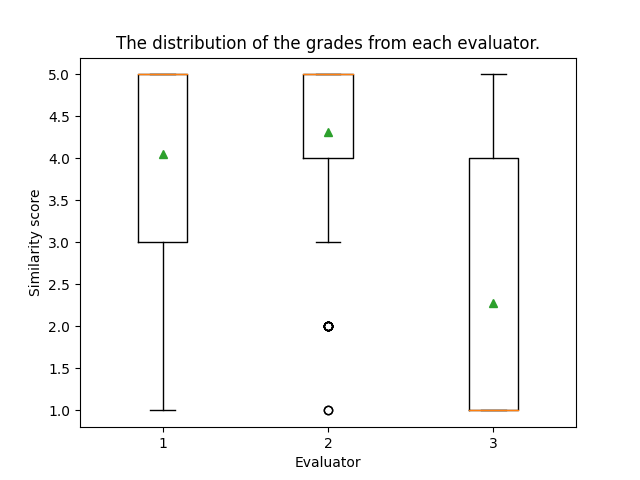
\includegraphics[width=\linewidth, height=6.5cm]{fig/fig.png}
    \caption{Box plot of evaluators on similarity of 100 sentence pairs paraphrased from the best model.}
    \label{fig:eval_res}
\end{figure}
As we can see in Figure \ref{fig:eval_res}, the results from the first two evaluators show the decent performance of the fine-tuned model.



\section*{Discussion}
In general, the performance of the model is very accurate on short sentences and paragraphs (ex. original sentence: "V slab\v{s}em polo\v{z}aju smo.", and paraphrased: "mi smo v slab\v{s}em polo\v{z}aju."). The model can perfectly handle numbers (ex. original sentence: "\v{s}tiri dolarje in 27 centov.", and paraphrased: "\v{s}tiri dolarje in sedemintrideset centov."). There were a lot of short sentences that were duplicated, mainly because of the fact that they were too short to be paraphrased. The models also can handle acronyms (ex. original sentence: "Uradni list Evropske unije L 210 z dne 31. julija 2006", and paraphrased: "(UL L 210, 31. julij 2006"). On the other hand, the model failed to paraphrase longer sentences, a common occurrence is to first successfully paraphrase the sentence and then add some meaningless random text, since the model failed to generate the "end of sentence" token. Also, the model uses the change of gender pronouns to paraphrase the original sentence which is not desirable.
% it works well on short sentences
%   V slabšem položaju smo. 
%   mi smo v slabšem položaju.

% alot of duplicated sentences
%   Rešitev je gospodarska rast. 
%   Rešitev je gospodarska rast.

% sometimes it returns weird random strings at the end of the paraphrase
%   Sodelovanje na področju boja proti terorizmu lahko poteka tudi s posameznimi državami, regijami ali mednarodnimi, regionalnimi ali podregionalnimi organizacijami; 
%   Sodelovanje v boju proti terorizmu se lahko vzpostavi tudi s posameznimi državami, regijami ali mednarodnimi, regionalnimi ali podregionalnimi organizacijami;pacocentriz ustavitspremljevalkaSchiff Združenj vrh Bocvandrobnosti bilančn

% there are a lot of law text
%   (Uradni list Evropske unije L 210 z dne 31. julija 2006) 
%   (UL L 210, 31. julij 2006)

% it can handle even numbers
%   štiri dolarje in sedemintrideset centov. 
%   štiri dolarje in 37 centov.


%\section*{Results}


\section*{Conclusion}
In conclusion, we obtained the data in the Slovenian language (by translation) for our research, trained a large language model such as GPT (Slovenian variant), and achieved decent performance which can be comparable with the paraphrasing models that are available for other lesser-known and utilized languages. Although the model has worse performance with longer sentences and paragraphs, it works very well on short sentences and paragraphs.
\subsection*{Future work}
Our next goal would be to improve our fine-tuned GPT model in terms of performance by selecting better fine-tuning parameters, obtaining a larger dataset (while also cleaning it more thoroughly), improving translations, and considering some other pre-trained large language models for text generation.
\par
In addition to the computational evaluation, we would like to improve the human evaluation by considering more instances for comparison which will give us less uncertainty in measuring the performance of our fine-tuned model.

%- make paraGPT better??
%- comp. eval: ROUGE and other scores
%- human eval: add syntax difference score

%----------------------------------------------------------------------------------------
%	REFERENCE LIST
%----------------------------------------------------------------------------------------
\bibliographystyle{unsrt}
\bibliography{report}


\end{document}
